\section*{\nr.3 \titthree (25 Punkte)}
\begin{enumerate}[(a)]
\item Mit 
\begin{equation}
  |\psi|^2=N^2x^2\exp\left(-\frac{x^2}{2\sigma^2}\right)
\end{equation}
folgt
\begin{equation}
  \int \mathrm{d}x |\psi|^2=N^2\sigma^3\sqrt{\frac{\pi}{4}}.
\end{equation}
Da dies gleich $1$ sein muss folgt
\begin{equation}
  N=\sqrt{\frac{2}{\sigma^3\sqrt{\pi}}}.
\end{equation}
\item Für den wahrscheinlichsten Aufenthaltsort muss gelten
\begin{equation}
  \frac{\mathrm{d}|\psi|^2}{\mathrm{d}x}=0.
\end{equation}
damit folgt
\begin{align}
  0&=2 N^2 x\exp\left(-\frac{x^2}{\sigma^2}\right) -\frac{2N^2}{\sigma^2}x^3\exp\left(-\frac{x^2}{\sigma^2}\right)\\
  &=2N^2x\exp\left(-\frac{x^2}{\sigma^2}\right)\left(1-\frac{x^2}{\sigma^2}\right)
\end{align}
Da $\frac{\mathrm{d}^2|\psi|^2}{\mathrm{d}x^2}(x=0)<0$ folgt, dass die Wahrscheinlichsten Aufenthaltsorte $x=\pm \sigma$ sind.
Der Mittelwert des Orts ergibt sich aus
\begin{equation}
  \langle x \rangle = \int \mathrm{d}x x|\psi|^2=0
\end{equation}
da man über das Produkt einer geraden und einer ungeraden Funktion integriert.\\
Eine Skizze der Wahrscheinlichkeitsdichte ist mit \vref{fig:plot} gegeben.
\begin{figure}[htbp]
\centering
% GNUPLOT: LaTeX picture with Postscript
\begingroup
  \makeatletter
  \providecommand\color[2][]{%
    \GenericError{(gnuplot) \space\space\space\@spaces}{%
      Package color not loaded in conjunction with
      terminal option `colourtext'%
    }{See the gnuplot documentation for explanation.%
    }{Either use 'blacktext' in gnuplot or load the package
      color.sty in LaTeX.}%
    \renewcommand\color[2][]{}%
  }%
  \providecommand\includegraphics[2][]{%
    \GenericError{(gnuplot) \space\space\space\@spaces}{%
      Package graphicx or graphics not loaded%
    }{See the gnuplot documentation for explanation.%
    }{The gnuplot epslatex terminal needs graphicx.sty or graphics.sty.}%
    \renewcommand\includegraphics[2][]{}%
  }%
  \providecommand\rotatebox[2]{#2}%
  \@ifundefined{ifGPcolor}{%
    \newif\ifGPcolor
    \GPcolorfalse
  }{}%
  \@ifundefined{ifGPblacktext}{%
    \newif\ifGPblacktext
    \GPblacktexttrue
  }{}%
  % define a \g@addto@macro without @ in the name:
  \let\gplgaddtomacro\g@addto@macro
  % define empty templates for all commands taking text:
  \gdef\gplbacktext{}%
  \gdef\gplfronttext{}%
  \makeatother
  \ifGPblacktext
    % no textcolor at all
    \def\colorrgb#1{}%
    \def\colorgray#1{}%
  \else
    % gray or color?
    \ifGPcolor
      \def\colorrgb#1{\color[rgb]{#1}}%
      \def\colorgray#1{\color[gray]{#1}}%
      \expandafter\def\csname LTw\endcsname{\color{white}}%
      \expandafter\def\csname LTb\endcsname{\color{black}}%
      \expandafter\def\csname LTa\endcsname{\color{black}}%
      \expandafter\def\csname LT0\endcsname{\color[rgb]{1,0,0}}%
      \expandafter\def\csname LT1\endcsname{\color[rgb]{0,1,0}}%
      \expandafter\def\csname LT2\endcsname{\color[rgb]{0,0,1}}%
      \expandafter\def\csname LT3\endcsname{\color[rgb]{1,0,1}}%
      \expandafter\def\csname LT4\endcsname{\color[rgb]{0,1,1}}%
      \expandafter\def\csname LT5\endcsname{\color[rgb]{1,1,0}}%
      \expandafter\def\csname LT6\endcsname{\color[rgb]{0,0,0}}%
      \expandafter\def\csname LT7\endcsname{\color[rgb]{1,0.3,0}}%
      \expandafter\def\csname LT8\endcsname{\color[rgb]{0.5,0.5,0.5}}%
    \else
      % gray
      \def\colorrgb#1{\color{black}}%
      \def\colorgray#1{\color[gray]{#1}}%
      \expandafter\def\csname LTw\endcsname{\color{white}}%
      \expandafter\def\csname LTb\endcsname{\color{black}}%
      \expandafter\def\csname LTa\endcsname{\color{black}}%
      \expandafter\def\csname LT0\endcsname{\color{black}}%
      \expandafter\def\csname LT1\endcsname{\color{black}}%
      \expandafter\def\csname LT2\endcsname{\color{black}}%
      \expandafter\def\csname LT3\endcsname{\color{black}}%
      \expandafter\def\csname LT4\endcsname{\color{black}}%
      \expandafter\def\csname LT5\endcsname{\color{black}}%
      \expandafter\def\csname LT6\endcsname{\color{black}}%
      \expandafter\def\csname LT7\endcsname{\color{black}}%
      \expandafter\def\csname LT8\endcsname{\color{black}}%
    \fi
  \fi
    \setlength{\unitlength}{0.0500bp}%
    \ifx\gptboxheight\undefined%
      \newlength{\gptboxheight}%
      \newlength{\gptboxwidth}%
      \newsavebox{\gptboxtext}%
    \fi%
    \setlength{\fboxrule}{0.5pt}%
    \setlength{\fboxsep}{1pt}%
\begin{picture}(7200.00,5040.00)%
    \gplgaddtomacro\gplbacktext{%
      \csname LTb\endcsname%
      \put(2318,484){\makebox(0,0){\strut{}$-\sigma$}}%
      \put(3600,484){\makebox(0,0){\strut{}$0$}}%
      \put(4881,484){\makebox(0,0){\strut{}$\sigma$}}%
    }%
    \gplgaddtomacro\gplfronttext{%
      \csname LTb\endcsname%
      \put(176,2739){\rotatebox{-270}{\makebox(0,0){\strut{}$|\psi|^2$}}}%
      \put(3599,154){\makebox(0,0){\strut{}$x$}}%
      \csname LTb\endcsname%
      \put(5816,4602){\makebox(0,0)[r]{\strut{}$|\psi|^2$}}%
    }%
    \gplbacktext
    \put(0,0){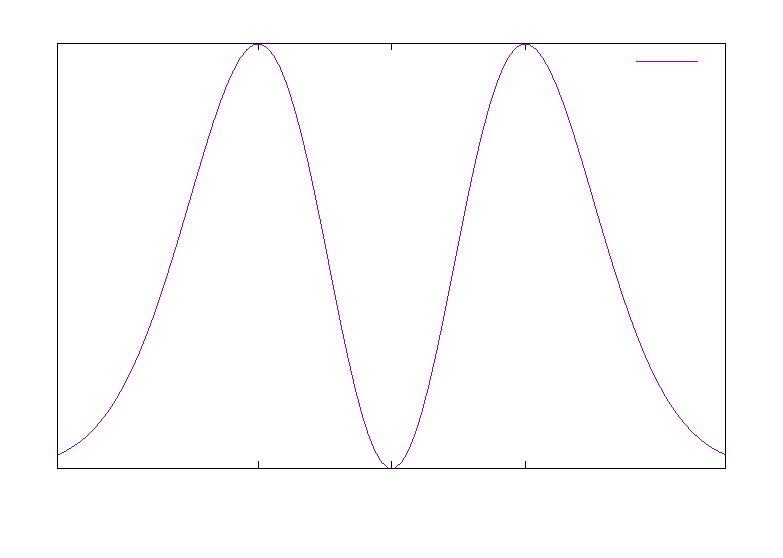
\includegraphics{plot}}%
    \gplfronttext
  \end{picture}%
\endgroup

\caption{Wahrscheinlichkeitsdichte der gegebenen Wellenfunktion}
\label{fig:plot}
\end{figure}

Es ist gut erkennbar, dass der Mittelwert des Teilchenorts der unwahrscheinlichste Aufenthaltsort des Teilchens ist. Auch wenn die Wahrscheinlichkeit für den Aufenthalt im Ursprung gleich Null ist, ist aufgrund der Symmetrie der Mittelwert trotzdem bei Null.

\end{enumerate}